\documentclass{article}

\usepackage{authblk} % for multiple authors and affiliations
\usepackage{graphicx} % to inlcude graphics with \includegraphics
\usepackage{tikz}
\usepackage{listings}
%\usepackage{geometry}
\usepackage[utf8]{inputenc}
\usepackage[T1]{fontenc}
\usepackage{fourier}


%New colors defined below
\definecolor{codegreen}{rgb}{0,0.6,0}
\definecolor{codegray}{rgb}{0.5,0.5,0.5}
\definecolor{codepurple}{rgb}{0.58,0,0.82}
\definecolor{backcolour}{rgb}{0.95,0.95,0.92}

%Code listing style named "mystyle"
\lstdefinestyle{mystyle}{
  backgroundcolor=\color{backcolour}, commentstyle=\color{codegreen},
  keywordstyle=\color{magenta},
  numberstyle=\tiny\color{codegray},
  stringstyle=\color{codepurple},
  basicstyle=\ttfamily\footnotesize,
  breakatwhitespace=false,         
  breaklines=true,                 
  captionpos=b,                    
  keepspaces=true,                 
  numbers=left,                    
  numbersep=5pt,                  
  showspaces=false,                
  showstringspaces=false,
  showtabs=false,                  
  tabsize=2
}

%"mystyle" code listing set
\lstset{style=mystyle}

\author{\textbf{MD ARIF HOSSAIN}}









\title{\textbf {The Generalization form of the order of an element in a group under addition modulo}}
%\affil{Department of Mathematics, Shahjalal University of Science and Technology, Sylhet, Bangladesh.}
\date{}

\begin{document}

\maketitle{}
%\tableofcontents


\section*{Abstract}

This paper explores the generalisation form of an element's order in a group under the addition modulo.We looked for an alternative approach to determine the order of an element within a group. We displayed the spiral-shaped graph to show how things are progressing. To prove that our alternate method is identical to the established approach , we have provided entire code.
\section{Introduction}

In mathematics, more specifically algebra, abstract algebra or modern algebra is the study of algebraic structures. Algebraic structures include groups, rings, fields, modules, vector spaces, lattices, and algebras over a field. The term abstract algebra was coined in the early 20th century to distinguish this area of study from older parts of algebra, and more specifically from elementary algebra, the use of variables to represent numbers in computation and reasoning.\cite{finston2014abstract}
\subsection{Group}
\subsubsection{Definition}
Let $G$ be a set together with a binary operation (usually called multiplication) that assigns to each ordered pair $(a, b)$ of elements of $G$ an element in $G$ denoted by $ab$.\\ We say G is a group under this operation if the following four properties are satisfied.\\
1.Closure: If $a$ and $b$ are two components in the group, $G$, then the product “$a * b$” is also in “$G$”.\\
2. Associativity: The operation is associative; that is, $(ab)c = a(bc)$ for
all $a, b, c$ in $G$.\\
3. Identity: There is an element e (called the identity) in $G$ such that
$ae = ea = a$ for all $a$ in $G$.\\
4. Inverses: For each element a in $G$, there is an element $b$ in $G$ (called
an inverse of $a$) such that $ab = ba = e$.\cite{gallian2021contemporary}




\subsection{Order of an element in a group}
\subsubsection{Definition}
The order of an element g in a group G is the smallest positive integer n
such that ($g^n$) = $e$. (In additive notation, this would be $ng$ = 0.) If no such
integer exists, we say that g has infinite order. The order of an element $g$
is denoted by $|g|$.\\
So, to find the order of a group element g, you need only compute the
sequence of products g, ($g^2$), ($g^3$) . . .  until you reach the identity for the first time. The exponent of this product (or coefficient if the operation is addition) is the order of g. If the identity never appears in the sequence, then
g has infinite order.\cite{gallian2021contemporary}
\subsection{Addition Modulo}
\subsubsection{Definition}
The word ‘modulo’ means ‘to the modulus’. For any positive integer $n$, let $S$ be the complete set of residues \{$0$, $1$, $2$,…, $n-1$\}. Then addition modulo $n$ on $S$ is defined as follows. For $a$ and $b$ in $S$, take the usual sum of $a$ and $b$ as integers, and let $r$ be the element of $S$ to which the result is congruent (modulo $n$); the sum $a+b$ (mod $n$) is equal to $r$. Similarly, multiplication modulo $n$ is defined by taking$ ab$ (mod $n$) to be equal to $s$, where $s$ is the element of $S$ to which the usual product of $a$ and $b$ is congruent (modulo $n$).\cite{clapham2014concise}
\subsection{L.C.M}
\subsubsection{Definition}
In arithmetic and number theory, the least common multiple, lowest common multiple, or smallest common multiple of two integers$ a $and $ b$, usually denoted by $lcm(a, b)$, is the smallest positive integer that is divisible by both a and b. Since division of integers by zero is undefined, this definition has meaning only if $a$ and $b$ are both different from zero. However, some authors define $lcm(a,0)$ as $0$ for all $a$, since $0$ is the only common multiple of $a$ and $0$ .\cite{hardy1979introduction}

\section{Method of Solving the problem}
For example,This is the conventional way to  \\
Consider $Z_{10}$ under addition modulo $10$. 
we know the residue class of $Z_{10}$ is $\{0,1,2,3,4,5,6,7,8,9\}$
Since $1 * 2 = 2$,
$2 * 2 = 4, 3 * 2 = 6, 4 * 2 = 8, 5 * 2 = 0$, we know that $|2| = 5$. \\
Similar computations  $|0| = 1, |7| = 10, |5| = 2, |6| = 5$.\\ (Here $2 * 2$ is an
abbreviation for $2 + 2, 3 * 2 $ is an abbreviation for $2 + 2 + 2$, etc.)\cite{gallian2021contemporary}\\\\
We can generate any modulo $Z n$ in a wheel setup to see how modular arithmetic works.We can pick any whole number $a$ in $Z_{10}$ to see which residue class it belongs.suppose we take $157$ so, $157 \equiv 7 mod (10)$ we can see its on the $[7] $ residue class.because we can derive $157 = 15*10 + 7$ which $10n+7$ which lied on the residue class $[7]$.In a wheel setup of modular arithmetic it its more easy to see the residue class of any number a. \\\\
\begin{center}
\begin{tikzpicture}[->,scale=.9]
   \node (a2) at (36:2cm)  {$2$};
   \node (b1) at (72:2cm) {$1$};
   \node (c) at (108:2cm) {$0$};
   \node (d) at (144:2cm)  {$9$};
   \node (e) at (180:2cm) {$8$};
   \node (f) at (216:2cm) {$7$};
   \node (g) at (252:2cm)  {$6$};
   \node (h) at (288:2cm) {$5$};
   \node (i) at (324:2cm) {$4$};
   \node (j) at (360:2cm) {$3$};
   \node (c) at (108:3cm) {$10$};
    \node (a) at (36:3cm)  {$12$};
   \node (b) at (72:3cm) {$11$};
   \node (c) at (108:4cm) {$20$};
   \node (d) at (144:3cm)  {$19$};
   \node (e) at (180:3cm) {$18$};
   \node (f) at (216:3cm) {$17$};
   \node (g) at (252:3cm)  {$16$};
   \node (h) at (288:3cm) {$15$};
   \node (i) at (324:3cm) {$14$};
   \node (j) at (360:3cm) {$13$};
   \node (c) at (108:5cm) {$30$};
     \node (a) at (36:4cm)  {$22$};
     \node (d) at (144:4cm)  {$29$};
     \node (e) at (180:4cm) {$28$};
   \node (f) at (216:4cm) {$27$};
   \node (g) at (252:4cm)  {$26$};
   \node (h) at (288:4cm) {$25$};
   \node (i) at (324:4cm) {$24$};
   \node (j) at (360:4cm) {$23$};
   \node (b) at (72:4cm) {$21$};
   \node (b) at (72:5cm) {$.$};
   \node (b) at (72:5.5cm) {$.$};
   \node (b) at (72:6cm) {$.$};
   \node (b) at (72:6.5cm) {$10n+1$};
   \node (a) at (36:5cm)  {$22$};
   \node (a) at (36:5.5cm)  {$.$};
   \node (a) at (36:6cm)  {$.$};
   \node (a) at (36:7cm)    {$10n+2$};
   \node (j) at (360:5cm) {$.$};
   \node (j) at (360:5.5cm) {$.$};
   \node (j) at (360:6.5cm) {$10n+3$};
   \node (i) at (324:5cm) {$.$};
   \node (i) at (324:5.5cm) {$.$};
   \node (i) at (324:6.5cm) {$10n+4$};
   \node (h) at (288:5cm) {$.$};
   \node (h) at (288:5.5cm) {$.$};
   \node (h) at (288:6cm) {$.$};
   \node (h) at (288:6.5cm) {$10n+5$};
   \node (g) at (252:5cm)  {$.$};
   \node (g) at (252:5.5cm)  {$.$};
   \node (g) at (252:6cm)  {$10n+6$};
   \node (f) at (216:5cm) {$.$};
   \node (f) at (216:5.5cm) {$.$};
   \node (f) at (216:7cm) {$10n+7$};
   \node (e) at (180:5cm) {$.$};
   \node (e) at (180:5.5cm) {$.$};
   \node (e) at (180:6.5cm)  {$10n+8$};
   \node (d) at (144:5cm)  {$.$};
   \node (d) at (144:5.5cm)  {$.$};
   \node (d) at (144:6.5cm)  {$10n+9$};
   \node (c) at (108:6cm) {$.$};
   \node (c) at (108:6.5cm) {$.$};
   \node (c) at (108:7cm) {$10n$};
   
     
    \end{tikzpicture}\\
    \end{center}
It's similar to a modulo $Z_{10}$ wheel setup.We can see all of the residue classes here$Z_{10}$=$\{[0],[1],[2],[3],[4],[5],[6],[7],[8],[9]\}$\\\\
In this case, $[0]$ represents the identity for the order of an element in a group under addition modulo.\\
And We know The order of an element g in a group G is the smallest positive integer n
such that ($g^n$) = $e$.\\
Here We need to start from $[0]$ to find the order of every element of this group.\\\\
So,The $0$ is already in the $[0]$ class and so the order of $0$ is 1\\\\
$ |0| = 1 $\\\\
For the element $1$ It will proceed to the residue class after exactly ten steps.\\\
\begin{center}
\begin{tikzpicture}[->,scale=.9]
   \node (a2) at (36:2cm)  {$2$};
   \node (a1) at (72:2cm) {$1$};
   \node (a0) at (108:2cm) {$0$};
   \node (a9) at (144:2cm)  {$9$};
   \node (a8) at (180:2cm) {$8$};
   \node (a7) at (216:2cm) {$7$};
   \node (a6) at (252:2cm)  {$6$};
   \node (a5) at (288:2cm) {$5$};
   \node (a4) at (324:2cm) {$4$};
   \node (a3) at (360:2cm) {$3$};
   \node (a10) at (108:3cm) {$10$};
   \path (a0) edge[bend left] (a1);
   \path (a1) edge[bend left] (a2);
   \path (a2) edge[bend left] (a3);
   \path (a3) edge[bend left] (a4);
   \path (a4) edge[bend left] (a5);
   \path (a5) edge[bend left] (a6);
   \path (a6) edge[bend left] (a7);
   \path (a7) edge[bend left] (a8);
   \path (a8) edge[bend left] (a9);
   \path (a9) edge[bend left] (a10);
   \path (a10) edge[] (a0);

\end{tikzpicture}\\
\end{center}
The steps will be counted as follows: 0 to 1 , 1 to 2 , 2 to 3 and so on.After exactly 10 bend arrows it moved to its identity element.the least amount of steps to be on residue class $[0]$ is $10$.Also in other words \\\\
the order of $1$ is 10\\\\

$ |1| = 10 $\\\\
For the element $2$ It will proceed to the residue class after exactly five steps.\\
\begin{center}
\begin{tikzpicture}[->,scale=.9]
   \node (a2) at (36:2cm)  {$2$};
   \node (a1) at (72:2.3cm) {$1$};
   \node (a0) at (108:2cm) {$0$};
   \node (a9) at (144:2.3cm)  {$9$};
   \node (a8) at (180:2cm) {$8$};
   \node (a7) at (216:2.3cm) {$7$};
   \node (a6) at (252:2cm)  {$6$};
   \node (a5) at (288:2.3cm) {$5$};
   \node (a4) at (324:2cm) {$4$};
   \node (a3) at (360:2.3cm) {$3$};
   \node (a10) at (108:3cm) {$10$};
   \path (a0) edge[bend left] (a2);
   \path (a2) edge[bend left] (a4);
   \path (a4) edge[bend left] (a6);
   \path (a6) edge[bend left] (a8);
   \path (a8) edge[bend left] (a10);
   
   \path (a10) edge[] (a0);

\end{tikzpicture}\\
\end{center}

The steps will be counted as follows: 0 to 2 , 2 to 4 , 4 to 6 and so on.the least amount of steps to be on residue class $[0]$ is $5$. $10$ , $20$ , $30$...also the multiple of $10$ or the residue class is [$0$] in $Z_10$ also the multiple of 2 too but the least common multiple of $2$ and $10$ is $10$.After exactly 5 bend arrows it moved to its identity element.Also in other words \\
the order of $2$ is $5$\\\\
$ |2| = 5 $.\\\\
For the element $3$ It will proceed to the residue class after exactly ten steps.\\
\begin{center}
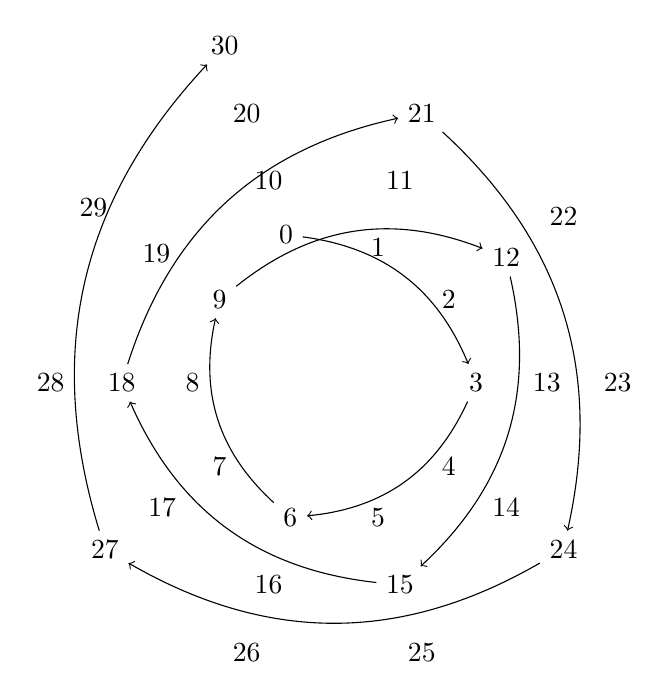
\begin{tikzpicture}[->,scale=.9]
   \node (a2) at (36:2cm)  {$2$};
   \node (a1) at (72:2cm) {$1$};
   \node (a0) at (108:2.2cm) {$0$};
   \node (a9) at (144:2cm)  {$9$};
   \node (a8) at (180:2cm) {$8$};
   \node (a7) at (216:2cm) {$7$};
   \node (a6) at (252:2cm)  {$6$};
   \node (a5) at (288:2cm) {$5$};
   \node (a4) at (324:2cm) {$4$};
   \node (a3) at (360:2cm) {$3$};
   \node (a10) at (108:3cm) {$10$};
   \node (a12) at (36:3cm)  {$12$};
   \node (a11) at (72:3cm) {$11$};
   \node (a20) at (108:4cm) {$20$};
   \node (a19) at (144:3.1cm)  {$19$};
   \node (a18) at (180:3cm) {$18$};
   \node (a17) at (216:3cm) {$17$};
   \node (a16) at (252:3cm)  {$16$};
   \node (a15) at (288:3cm) {$15$};
   \node (a14) at (324:3cm) {$14$};
   \node (a13) at (360:3cm) {$13$};
   \node (a30) at (108:5cm) {$30$};
     \node (a22) at (36:4cm)  {$22$};
     \node (a29) at (144:4.2cm)  {$29$};
     \node (a28) at (180:4cm) {$28$};
   \node (a27) at (216:4cm) {$27$};
   \node (a26) at (252:4cm)  {$26$};
   \node (a25) at (288:4cm) {$25$};
   \node (a24) at (324:4cm) {$24$};
   \node (a23) at (360:4cm) {$23$};
   \node (a21) at (72:4cm) {$21$};


   \path (a0) edge[bend left] (a3);
   \path (a3) edge[bend left] (a6);
   \path (a6) edge[bend left] (a9);
   \path (a9) edge[bend left] (a12);
   \path (a12) edge[bend left] (a15);
   \path (a15) edge[bend left] (a18);
   \path (a18) edge[bend left] (a21);
   \path (a21) edge[bend left] (a24);
   \path (a24) edge[bend left] (a27);
   \path (a27) edge[bend left] (a30);
  % \path (a30) edge[bend left] (a0);

\end{tikzpicture}\\
\end{center}
The steps will be counted as follows: 0 to 3 , 3 to 6 , 6 to 9 and so on.After exactly 10 bend arrows it moved to its identity element..the least amount of steps to be on residue class $[3]$ is $10$.Also in other words, \\
the order of $3$ is $10$\\\\
$ |3| = 10 $\\\\
This will be continue for every other element of $Z_{10}$\\\\
\begin{center}
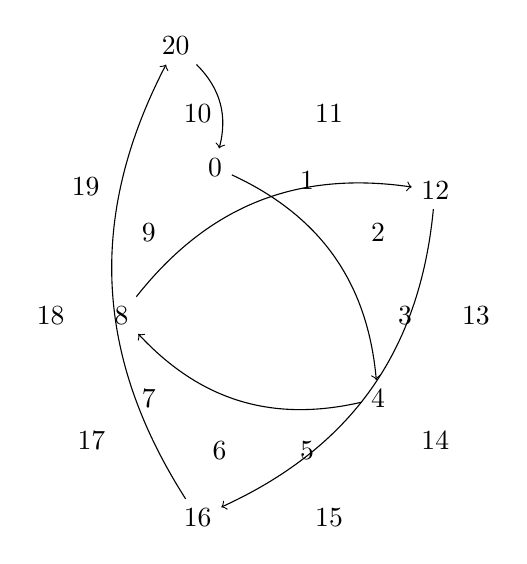
\begin{tikzpicture}[->,scale=.9]
   \node (a2) at (36:2cm)  {$2$};
   \node (a1) at (72:2cm) {$1$};
   \node (a0) at (108:2.2cm) {$0$};
   \node (a9) at (144:2cm)  {$9$};
   \node (a8) at (180:2cm) {$8$};
   \node (a7) at (216:2cm) {$7$};
   \node (a6) at (252:2cm)  {$6$};
   \node (a5) at (288:2cm) {$5$};
   \node (a4) at (324:2cm) {$4$};
   \node (a3) at (360:2cm) {$3$};
   \node (a10) at (108:3cm) {$10$};
   \node (a12) at (36:3cm)  {$12$};
   \node (a11) at (72:3cm) {$11$};
   \node (a20) at (108:4cm) {$20$};
   \node (a19) at (144:3.1cm)  {$19$};
   \node (a18) at (180:3cm) {$18$};
   \node (a17) at (216:3cm) {$17$};
   \node (a16) at (252:3cm)  {$16$};
   \node (a15) at (288:3cm) {$15$};
   \node (a14) at (324:3cm) {$14$};
   \node (a13) at (360:3cm) {$13$};

   \path (a0) edge[bend left] (a4);
   \path (a4) edge[bend left] (a8);
   \path (a8) edge[bend left] (a12);
   \path (a12) edge[bend left] (a16);
   \path (a16) edge[bend left] (a20);
   
  \path (a20) edge[bend left] (a0);

\end{tikzpicture}\\
\end{center}
The steps will be counted as follows: 0 to 4 , 4 to 8 , 8 to 12 and so on.After exactly 5 bend arrows it moved to its identity element..the least amount of steps to be on residue class $[4]$ is $5$.Also in other words, \\
the order of $4$ is $5$\\\\
$ |4| = 5 $\\\\
\begin{center}
\begin{tikzpicture}[->,scale=.9]
   \node (a2) at (36:2cm)  {$2$};
   \node (a1) at (72:2cm) {$1$};
   \node (a0) at (108:2.2cm) {$0$};
   \node (a9) at (144:2cm)  {$9$};
   \node (a8) at (180:2cm) {$8$};
   \node (a7) at (216:2cm) {$7$};
   \node (a6) at (252:2cm)  {$6$};
   \node (a5) at (288:2cm) {$5$};
   \node (a4) at (324:2cm) {$4$};
   \node (a3) at (360:2cm) {$3$};
   \node (a10) at (108:3cm) {$10$};


   \path (a0) edge[bend left] (a5);
   \path (a5) edge[bend left] (a10);
   
   \path (a10) edge[] (a0);
   
   \end{tikzpicture}\\
\end{center}
The steps will be counted as follows: 0 to 5 , 5 to 10 After exactly 2 bend arrows it moved to its identity element..the least amount of steps to be on residue class $[5]$ is $2$.Also in other words, \\
the order of $5$ is $2$\\\\
$ |5| = 2 $\\\\
\begin{center}
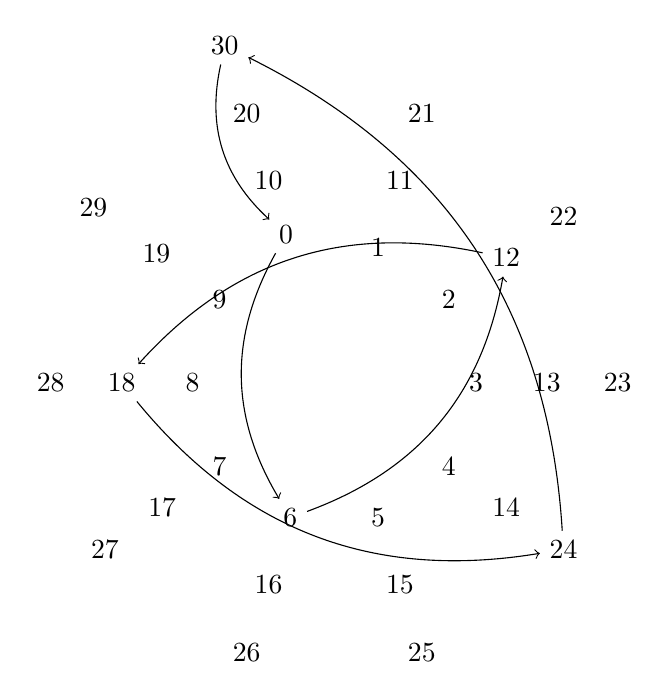
\begin{tikzpicture}[->,scale=.9]
   \node (a2) at (36:2cm)  {$2$};
   \node (a1) at (72:2cm) {$1$};
   \node (a0) at (108:2.2cm) {$0$};
   \node (a9) at (144:2cm)  {$9$};
   \node (a8) at (180:2cm) {$8$};
   \node (a7) at (216:2cm) {$7$};
   \node (a6) at (252:2cm)  {$6$};
   \node (a5) at (288:2cm) {$5$};
   \node (a4) at (324:2cm) {$4$};
   \node (a3) at (360:2cm) {$3$};
   \node (a10) at (108:3cm) {$10$};
   \node (a12) at (36:3cm)  {$12$};
   \node (a11) at (72:3cm) {$11$};
   \node (a20) at (108:4cm) {$20$};
   \node (a19) at (144:3.1cm)  {$19$};
   \node (a18) at (180:3cm) {$18$};
   \node (a17) at (216:3cm) {$17$};
   \node (a16) at (252:3cm)  {$16$};
   \node (a15) at (288:3cm) {$15$};
   \node (a14) at (324:3cm) {$14$};
   \node (a13) at (360:3cm) {$13$};
   \node (a30) at (108:5cm) {$30$};
     \node (a22) at (36:4cm)  {$22$};
     \node (a29) at (144:4.2cm)  {$29$};
     \node (a28) at (180:4cm) {$28$};
   \node (a27) at (216:4cm) {$27$};
   \node (a26) at (252:4cm)  {$26$};
   \node (a25) at (288:4cm) {$25$};
   \node (a24) at (324:4cm) {$24$};
   \node (a23) at (360:4cm) {$23$};
   \node (a21) at (72:4cm) {$21$};


   \path (a0) edge[bend right] (a6);
   \path (a6) edge[bend right] (a12);
   \path (a12) edge[bend right] (a18);
   \path (a18) edge[bend right] (a24);
   \path (a24) edge[bend right] (a30);
  \path (a30) edge[bend right] (a0);

\end{tikzpicture}\\
\end{center}
The steps will be counted as follows: 0 to 6 , 6 to 12 , 12 to 18 and so on.After exactly 5 bend arrows it moved to its identity element..the least amount of steps to be on residue class $[6]$ is $5$.Also in other words, \\
the order of $6$ is $5$\\\\
$ |6| = 5 $\\\\
\begin{center}
\begin{tikzpicture}[->,scale=.9]
   \node (a2) at (36:2cm)  {$2$};
   \node (a1) at (72:2cm) {$1$};
   \node (a0) at (108:2.2cm) {$0$};
   \node (a9) at (144:2cm)  {$9$};
   \node (a8) at (180:2cm) {$8$};
   \node (a7) at (216:2cm) {$7$};
   \node (a6) at (252:2cm)  {$6$};
   \node (a5) at (288:2cm) {$5$};
   \node (a4) at (324:2cm) {$4$};
   \node (a3) at (360:2cm) {$3$};
   \node (a10) at (108:3cm) {$10$};
   \node (a12) at (36:3cm)  {$12$};
   \node (a11) at (72:3cm) {$11$};
   \node (a20) at (108:4cm) {$20$};
   \node (a19) at (144:3.1cm)  {$19$};
   \node (a18) at (180:3cm) {$18$};
   \node (a17) at (216:3cm) {$17$};
   \node (a16) at (252:3cm)  {$16$};
   \node (a15) at (288:3cm) {$15$};
   \node (a14) at (324:3cm) {$14$};
   \node (a13) at (360:3cm) {$13$};
   
   \node (a21) at (72:4cm) {$21$};
    \node (a22) at (36:4cm)  {$22$};
    \node (a23) at (360:4cm) {$23$};
    \node (a24) at (324:4cm) {$24$};
    \node (a25) at (288:4cm) {$25$};
    \node (a26) at (252:4cm)  {$26$};
    \node (a27) at (216:4cm) {$27$};
    \node (a28) at (180:4cm) {$28$};
    \node (a29) at (144:4.2cm)  {$29$};
    \node (a30) at (108:5cm) {$30$};

 \node (a31) at (72:5cm) {$31$};
    \node (a32) at (36:5cm)  {$32$};
    \node (a3) at (360:5cm) {$33$};
    \node (a34) at (324:5cm) {$34$};
    \node (a35) at (288:5cm) {$35$};
    \node (a36) at (252:5cm)  {$36$};
    \node (a37) at (216:5cm) {$37$};
    \node (a38) at (180:5cm) {$38$};
    \node (a39) at (144:5.2cm)  {$39$};
    \node (a40) at (108:6cm) {$40$};


     \node (a41) at (72:6cm) {$41$};
    \node (a42) at (36:6cm)  {$42$};
    \node (a43) at (360:6cm) {$43$};
    \node (a44) at (324:6cm) {$44$};
    \node (a45) at (288:6cm) {$45$};
    \node (a46) at (252:6cm)  {$46$};
    \node (a47) at (216:6cm) {$47$};
    \node (a48) at (180:6cm) {$48$};
    \node (a49) at (144:6cm)  {$49$};
    \node (a50) at (108:7cm) {$50$};


    \node (a51) at (72:7cm) {$51$};
    \node (a52) at (36:7cm)  {$52$};
    \node (a53) at (360:7cm) {$53$};
    \node (a54) at (324:7cm) {$54$};
    \node (a55) at (288:7cm) {$55$};
    \node (a56) at (252:7cm)  {$56$};
    \node (a57) at (216:7cm) {$57$};
    \node (a58) at (180:7cm) {$58$};
    \node (a59) at (144:7cm)  {$59$};
    \node (a60) at (108:8cm) {$60$};


    
    \node (a61) at (72:8cm) {$61$};
    \node (a62) at (36:8cm)  {$62$};
    \node (a63) at (360:8cm) {$63$};
    \node (a64) at (324:8cm) {$64$};
    \node (a65) at (288:8cm) {$65$};
    \node (a66) at (252:8cm)  {$66$};
    \node (a67) at (216:8cm) {$67$};
    \node (a68) at (180:8cm) {$68$};
    \node (a69) at (144:8cm)  {$69$};
    \node (a70) at (108:9cm) {$70$};
    
  
   
   
   
   \path (a0) edge[bend right] (a7);
   \path (a7) edge[bend right] (a14);
   \path (a14) edge[bend right] (a21);
   \path (a21) edge[bend right] (a28);
   \path (a28) edge[bend right] (a35);
  \path (a35) edge[bend right] (a42);
   \path (a42) edge[bend right] (a49);
   \path (a49) edge[bend right] (a56);
   \path (a56) edge[bend right] (a63);
   \path (a63) edge[bend right] (a70);
  \path (a70) edge[bend right] (a0);

\end{tikzpicture}\\
\end{center}
The steps will be counted as follows: 0 to 7 , 7 to 14 , 14 to 21 and so on.After exactly 10 bend arrows it moved to its identity element..the least amount of steps to be on residue class $[7]$ is $10$.Also in other words, \\
the order of $7$ is $10$\\\\
$ |7| = 10 $\\\\
\begin{center}
\begin{tikzpicture}[->,scale=.9]
   \node (a2) at (36:2cm)  {$2$};
   \node (a1) at (72:2cm) {$1$};
   \node (a0) at (108:2.2cm) {$0$};
   \node (a9) at (144:2cm)  {$9$};
   \node (a8) at (180:2cm) {$8$};
   \node (a7) at (216:2cm) {$7$};
   \node (a6) at (252:2cm)  {$6$};
   \node (a5) at (288:2cm) {$5$};
   \node (a4) at (324:2cm) {$4$};
   \node (a3) at (360:2cm) {$3$};
   \node (a10) at (108:3cm) {$10$};
   \node (a12) at (36:3cm)  {$12$};
   \node (a11) at (72:3cm) {$11$};
   \node (a20) at (108:4cm) {$20$};
   \node (a19) at (144:3.1cm)  {$19$};
   \node (a18) at (180:3cm) {$18$};
   \node (a17) at (216:3cm) {$17$};
   \node (a16) at (252:3cm)  {$16$};
   \node (a15) at (288:3cm) {$15$};
   \node (a14) at (324:3cm) {$14$};
   \node (a13) at (360:3cm) {$13$};
   
   \node (a21) at (72:4cm) {$21$};
    \node (a22) at (36:4cm)  {$22$};
    \node (a23) at (360:4cm) {$23$};
    \node (a24) at (324:4cm) {$24$};
    \node (a25) at (288:4cm) {$25$};
    \node (a26) at (252:4cm)  {$26$};
    \node (a27) at (216:4cm) {$27$};
    \node (a28) at (180:4cm) {$28$};
    \node (a29) at (144:4.2cm)  {$29$};
    \node (a30) at (108:5cm) {$30$};

 \node (a31) at (72:5cm) {$31$};
    \node (a32) at (36:5cm)  {$32$};
    \node (a3) at (360:5cm) {$33$};
    \node (a34) at (324:5cm) {$34$};
    \node (a35) at (288:5cm) {$35$};
    \node (a36) at (252:5cm)  {$36$};
    \node (a37) at (216:5cm) {$37$};
    \node (a38) at (180:5cm) {$38$};
    \node (a39) at (144:5.2cm)  {$39$};
    \node (a40) at (108:6cm) {$40$};

    
   \path (a0) edge[bend right] (a8);
   \path (a8) edge[bend right] (a16);
   \path (a16) edge[bend right] (a24);
   \path (a24) edge[bend right] (a32);
   \path (a32) edge[bend right] (a40);
   
  \path (a40) edge[bend right] (a0);

    \end{tikzpicture}
    \end{center}
The steps will be counted as follows: 0 to 8 , 8 to 16 , 16 to 24 and so on.After exactly 5 bend arrows it moved to its identity element..the least amount of steps to be on residue class $[8]$ is $5$.Also in other words, \\
the order of $8$ is $5$\\\\

$ |8| = 5 $\\\\

\begin{center}
\begin{tikzpicture}[->,scale=.9]
   \node (a2) at (36:1cm)  {$2$};
   \node (a1) at (72:1cm) {$1$};
   \node (a0) at (108:1cm) {$0$};
   \node (a9) at (144:1cm)  {$9$};
   \node (a8) at (180:1cm) {$8$};
   \node (a7) at (216:1cm) {$7$};
   \node (a6) at (252:1cm)  {$6$};
   \node (a5) at (288:1cm) {$5$};
   \node (a4) at (324:1cm) {$4$};
   \node (a3) at (360:1cm) {$3$};
   \node (a10) at (108:2cm) {$10$};
   \node (a12) at (36:2cm)  {$12$};
   \node (a11) at (72:2cm) {$11$};
   \node (a20) at (108:3cm) {$20$};
   \node (a19) at (144:2cm)  {$19$};
   \node (a18) at (180:2cm) {$18$};
   \node (a17) at (216:2cm) {$17$};
   \node (a16) at (252:2cm)  {$16$};
   \node (a15) at (288:2cm) {$15$};
   \node (a14) at (324:2cm) {$14$};
   \node (a13) at (360:2cm) {$13$};
   
   \node (a21) at (72:3cm) {$21$};
    \node (a22) at (36:3cm)  {$22$};
    \node (a23) at (360:3cm) {$23$};
    \node (a24) at (324:3cm) {$24$};
    \node (a25) at (288:3cm) {$25$};
    \node (a26) at (252:3cm)  {$26$};
    \node (a27) at (216:3cm) {$27$};
    \node (a28) at (180:3cm) {$28$};
    \node (a29) at (144:3cm)  {$29$};
    \node (a30) at (108:4cm) {$30$};

 \node (a31) at (72:4cm) {$31$};
    \node (a32) at (36:4cm)  {$32$};
    \node (a3) at (360:4cm) {$33$};
    \node (a34) at (324:4cm) {$34$};
    \node (a35) at (288:4cm) {$35$};
    \node (a36) at (252:4cm)  {$36$};
    \node (a37) at (216:4cm) {$37$};
    \node (a38) at (180:4cm) {$38$};
    \node (a39) at (144:4cm)  {$39$};
    \node (a40) at (108:5cm) {$40$};


     \node (a41) at (72:5cm) {$41$};
    \node (a42) at (36:5cm)  {$42$};
    \node (a43) at (360:5cm) {$43$};
    \node (a44) at (324:5cm) {$44$};
    \node (a45) at (288:5cm) {$45$};
    \node (a46) at (252:5cm)  {$46$};
    \node (a47) at (216:5cm) {$47$};
    \node (a48) at (180:5cm) {$48$};
    \node (a49) at (144:5cm)  {$49$};
    \node (a50) at (108:6cm) {$50$};


    \node (a51) at (72:6cm) {$51$};
    \node (a52) at (36:6cm)  {$52$};
    \node (a53) at (360:6cm) {$53$};
    \node (a54) at (324:6cm) {$54$};
    \node (a55) at (288:6cm) {$55$};
    \node (a56) at (252:6cm)  {$56$};
    \node (a57) at (216:6cm) {$57$};
    \node (a58) at (180:6cm) {$58$};
    \node (a59) at (144:6cm)  {$59$};
    \node (a60) at (108:7cm) {$60$};


    
    \node (a61) at (72:7cm) {$61$};
    \node (a62) at (36:7cm)  {$62$};
    \node (a63) at (360:7cm) {$63$};
    \node (a64) at (324:7cm) {$64$};
    \node (a65) at (288:7cm) {$65$};
    \node (a66) at (252:7cm)  {$66$};
    \node (a67) at (216:7cm) {$67$};
    \node (a68) at (180:7cm) {$68$};
    \node (a69) at (144:7cm)  {$69$};
    \node (a70) at (108:8cm) {$70$};

    \node (a71) at (72:8cm)  {$71$};
    \node (a72) at (36:8cm)  {$72$};
    \node (a73) at (360:8cm) {$73$};
    \node (a74) at (324:8cm) {$74$};
    \node (a75) at (288:8cm) {$75$};
    \node (a76) at (252:8cm) {$76$};
    \node (a77) at (216:8cm) {$77$};
    \node (a78) at (180:8cm) {$78$};
    \node (a79) at (144:8cm) {$79$};
    \node (a80) at (108:9cm) {$80$};

    \node (a81) at (72:9cm)  {$81$};
    \node (a82) at (36:9cm)  {$82$};
    \node (a83) at (360:9cm) {$83$};
    \node (a84) at (324:9cm) {$84$};
    \node (a85) at (288:9cm) {$85$};
    \node (a86) at (252:9cm) {$86$};
    \node (a87) at (216:9cm) {$87$};
    \node (a88) at (180:9cm) {$88$};
    \node (a89) at (144:9cm) {$89$};
    \node (a90) at (108:10cm) {$90$};
    
  
   
   
   
   \path (a0) edge[bend right] (a9);
   \path (a9) edge[bend right] (a18);
   \path (a18) edge[bend right] (a27);
   \path (a27) edge[bend right] (a36);
   \path (a36) edge[bend right] (a45);
  \path (a45) edge[bend right] (a54);
   \path (a54) edge[bend right] (a63);
   \path (a63) edge[bend right] (a72);
   \path (a72) edge[bend right] (a81);
   \path (a81) edge[bend right] (a90);
  \path (a90) edge[bend right] (a0);

\end{tikzpicture}\\
\end{center}
The steps will be counted as follows: 0 to 9 , 9 to 18 , 18 to 27 and so on.After exactly 10 bend arrows it moved to its identity element..the least amount of steps to be on residue class $[9]$ is $10$.Also in other words, \\
the order of $9$ is $10$\\\\

$ |9| = 10 $\\\\
We can clearly see a pattern here, A element takes the fewest steps to travel residue class $[0]$ is the order of that element.in residue class $[0]$=\{10 , 20, 30 , 40 , 50 , 60  ...$10*n$\} where n $\geq$0 and $n \in N$ which is the element's common multiple, and $Z_n$\\\\
As a result, the shortest step is and the element in n $\geq$ 0\\\\
$|1|$ = $\frac{l.c.m (1,10)}{1} ={\frac{10}{1}} = 10$\\\\
$|2|$ = $\frac{l.c.m (2,10)}{2} ={\frac{10}{2}} =5$\\\\
$|3|$ = $\frac{l.c.m (3,10)}{3} ={\frac{30}{3}} = 10$\\\\
$|4|$ = $\frac{l.c.m (4,10)}{4} ={\frac{20}{4}} = 5$\\\\
$|5|$ = $\frac{l.c.m (5,10)}{5} ={\frac{10}{5}} = 2$\\\\
$|6|$ = $\frac{l.c.m (6,10)}{6} ={\frac{30}{6}} = 5$\\\\
$|7|$ = $\frac{l.c.m (7,10)}{7} ={\frac{70}{7}} = 10$\\\\
$|8|$ = $\frac{l.c.m (8,10)}{8} ={\frac{40}{8}} = 5$\\\\
$|9|$ = $\frac{l.c.m (9,10)}{9} ={\frac{90}{9}} = 10$\\\\
Thus we have found the fewest steps.\\\\
If the element and addition modulo is relatively prime to $Z_n$,then that element's order is $n$\\\\
\section{The Generalization form}
\subsection{Theorem}
Under addition modulo $Z_n$, the order of an element in a group is for each element to take the least number of steps to go to the identity residue class which is $[0]$.The order of element $a$ in $Z_n$ is  ${\frac{l.c.m(a,n)}{a}}$ where $0<a\le n-1$.\\\

\subsubsection{Proof}
Let's take the addition modulo $Z_n$ and its residue classes are $Z_{n}$=$\{[0],[1],[2],[3],[4],[5],[6],[7],[8],....,[n-1]\}$ \\\\
and order of each element under $Z_n$ is $Z_n =\{0,1,2,3,4,5,6,7.....,(n-1)\}$\\\\
Here,the identity for the addition modulo is residue class $[0]$ and the element $0$ is already in the residue class $1$ so the order is $1$ but for n $\geq 0$ the order of that element\\\\

Now lets,take $Z_2$ so here the residue class are =$\{[0],[1]\}$ and the elements are $Z_2$=$\{0,1\}$\\\\


so the order of $0$ is $1$\\\\
the order of $1$ is\\\\
$|1|$ = $\frac{l.c.m (1,2)}{1} = 2$\\\\
\begin{center}
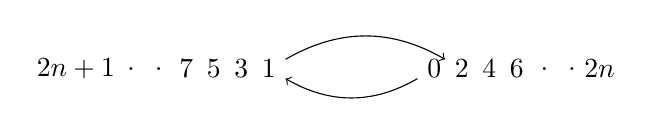
\begin{tikzpicture}[->,scale=.7]
\node (i0) at (0:1cm)  {$0$};
   \node (i1) at (180:2cm) {$1$};
   \node (i2) at (0:1.5cm)  {$2$};
   \node (j) at (180:2.5cm) {$3$};
   \node (i) at (0:2cm)  {$4$};
   \node (j) at (180:3cm) {$5$};
   \node (i) at (0:2.5cm)  {$6$};
   \node (j) at (180:3.5cm) {$7$};
   \node (i) at (0:3cm)  {$.$};
   \node (j) at (180:4cm) {$.$};
   \node (i) at (0:3.5cm)  {$.$};
   \node (j) at (180:4.5cm) {$.$};
   \node (i) at (0:4cm)  {$2n$};
   \node (j) at (180:5.5cm) {$2n+1$};
   \path (i0) edge[bend left] (i1);
   \path (i1) edge[bend left] (i2);
   
   \end{tikzpicture}\\
   \end{center}
Now lets,take $Z_3$ so here the residue class are =$\{[0],[1],[2]\}$ and the elements are $Z_3$=$\{0,1,2\}$\\\\
\begin{center}
    \begin{tikzpicture}[->,scale=.7]
   \node (i) at (90:1cm)  {$0$};
   \node (j) at (-30:1cm) {$1$};
   \node (k) at (210:1cm) {$2$};
   \node (i) at (90:2cm)  {$3$};
   \node (j) at (-30:2cm) {$4$};
   \node (k) at (210:2cm) {$5$};
   \node (i) at (90:3cm)  {$6$};
   \node (j) at (-30:3cm) {$7$};
   \node (k) at (210:3cm) {$8$};
   \node (i) at (90:3.5cm)  {$.$};
   \node (j) at (-30:3.5cm) {$.$};
   \node (k) at (210:3.5cm) {$.$};
   \node (i) at (90:4cm)  {$.$};
   \node (j) at (-30:4cm) {$.$};
   \node (k) at (210:4cm) {$.$};
   \node (i) at (90:4.5cm)  {$3n$};
   \node (j) at (-30:5cm) {$3n+1$};
   \node (k) at (210:5cm) {$3n+2$};
\end{tikzpicture}\\
\end{center}

the order of $0$ is $1$ always.\\\\
\begin{center}
    \begin{tikzpicture}[->,scale=.7]
   \node (a0) at (90:1cm)  {$0$};
   \node (a1) at (-30:1cm) {$1$};
   \node (a2) at (210:1cm) {$2$};
   \node (a3) at (90:2cm)  {$3$};
   \node (a4) at (-30:2cm) {$4$};
   \node (a5) at (210:2cm) {$5$};
   \node (a6) at (90:3cm)  {$6$};

    \path (a0) edge[bend left] (a1);
   \path (a1) edge[bend left] (a2);
   \path (a2) edge[bend left] (a3);
    \path (a3) edge[] (a0);
   

\end{tikzpicture}\\
\end{center}
The order of $1$ is $|1|$ = $\frac{l.c.m (1,3)}{1} = 3$\\\\
\begin{center}
    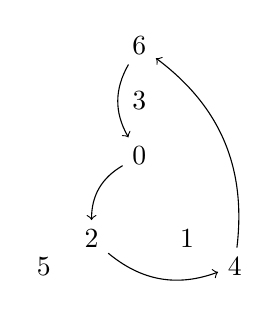
\begin{tikzpicture}[->,scale=.7]
   \node (a0) at (90:1cm)  {$0$};
   \node (a1) at (-30:1cm) {$1$};
   \node (a2) at (210:1cm) {$2$};
   \node (a3) at (90:2cm)  {$3$};
   \node (a4) at (-30:2cm) {$4$};
   \node (a5) at (210:2cm) {$5$};
   \node (a6) at (90:3cm)  {$6$};

    \path (a0) edge[bend right] (a2);
   \path (a2) edge[bend right] (a4);
   \path (a4) edge[bend right] (a6);
    \path (a6) edge[bend right] (a0);
   

\end{tikzpicture}\\
\end{center}
The order of $2$ is $|2|$ = $\frac{l.c.m (2,3)}{2} = 3$\\\\
let's take a prime number like $Z_n$ where $n$ is any prime number for now suppose $n=7$ so the residue class are $Z_7$=$\{[0],[1],[2],[3],[4],[5],[6]$\}\\\\
\begin{center}
    \begin{tikzpicture}[->,scale=.7]
   \node (a) at (51.42:2cm)  {$0$};
   \node (b) at (102.42:2cm) {$6$};
   \node (c) at (154.26:2cm) {$5$};
   \node (d) at (205.68:2cm)  {$4$};
   \node (e) at (257.1:2cm) {$3$};
   \node (f) at (308.52:2cm) {$2$};
   \node (g) at (359.94:2.5cm)  {$1$};
   
   
   \node (a) at (51.42:3cm)  {$7$};
   \node (b) at (102.42:3cm) {$13$};
   \node (c) at (154.26:3cm) {$12$};
   \node (d) at (205.68:3cm)  {$11$};
   \node (e) at (257.1:3cm) {$10$};
   \node (f) at (308.52:3cm) {$9$};
   \node (g) at (359.94:3cm)  {$8$};
   
   
   
   \node (a) at (51.42:4cm)  {$.$};
   \node (b) at (102.42:4cm) {$.$};
   \node (c) at (154.26:4cm) {$.$};
   \node (d) at (205.68:4cm)  {$.$};
   \node (e) at (257.1:4cm) {$.$};
   \node (f) at (308.52:4cm) {$.$};
   \node (g) at (359.94:4cm)  {$.$};
   
   
    \node (a) at (51.42:5cm)  {$7n$};
   \node (b) at (102.42:5cm) {$7n+6$};
   \node (c) at (154.26:5cm) {$7n+5$};
   \node (d) at (205.68:5cm)  {$7n+4$};
   \node (e) at (257.1:5cm) {$7n+3$};
   \node (f) at (308.52:5cm) {$7n+2$};
   \node (g) at (359.94:5cm)  {$7n+1$};
   \end{tikzpicture}\\\
\end{center}

   We Know the order of $|0|$ is 1 and the rest is \\\\
   %for 1 mod 7 type
\begin{center}
    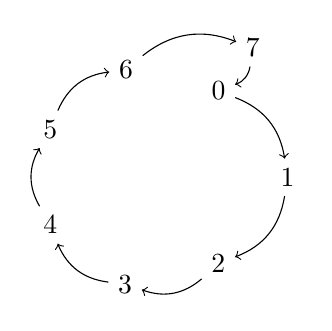
\begin{tikzpicture}[->,scale=.7]
   \node (a0) at (51.42:2cm)  {$0$};
   \node (a6) at (102.42:2cm) {$6$};
   \node (a5) at (154.26:2cm) {$5$};
   \node (a4) at (205.68:2cm)  {$4$};
   \node (a3) at (257.1:2cm) {$3$};
   \node (a2) at (308.52:2cm) {$2$};
   \node (a1) at (359.94:2.5cm)  {$1$};
    \node (a7) at (51.42:3cm)  {$7$};
    
      \path (a0) edge[bend left] (a1);
   \path (a1) edge[bend left] (a2);
   \path (a2) edge[bend left] (a3);
   \path (a3) edge[bend left] (a4);
   \path (a4) edge[bend left] (a5);
   \path (a5) edge[bend left] (a6);
   \path (a6) edge[bend left] (a7);
   \path (a7) edge[bend left] (a0);
    \end{tikzpicture}\\\
\end{center}
   
   $|1|$ = $\frac{l.c.m (1,7)}{1} ={\frac{10}{1}} = 7$\\\\
   %%for 2 mod 7 type
\begin{center}
    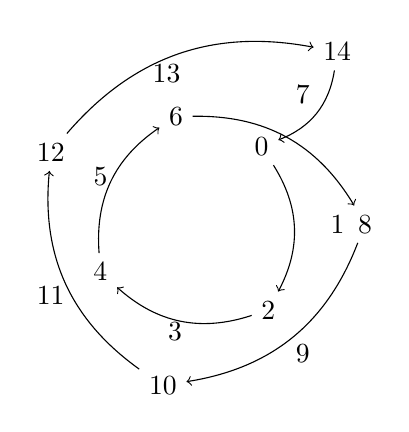
\begin{tikzpicture}[->,scale=.7]
   \node (a0) at (51.42:1.8cm)  {$0$};
   \node (a6) at (102.42:2cm) {$6$};
   \node (a5) at (154.26:2cm) {$5$};
   \node (a4) at (205.68:2cm)  {$4$};
   \node (a3) at (257.1:2cm) {$3$};
   \node (a2) at (308.52:2cm) {$2$};
   \node (a1) at (359.94:2.5cm)  {$1$};
    \node (a7) at (51.42:3cm)  {$7$};
    \node (a13) at (102.42:2.8cm) {$13$};
   \node (a12) at (154.26:3cm) {$12$};
   \node (a11) at (205.68:3cm)  {$11$};
   \node (a10) at (257.1:3cm) {$10$};
   \node (a9) at (308.52:3cm) {$9$};
   \node (a8) at (359.94:3cm)  {$8$};
   \node (a14) at (51.42:4cm)  {$14$};
    
      \path (a0) edge[bend left] (a2);
   \path (a2) edge[bend left] (a4);
   \path (a4) edge[bend left] (a6);
   \path (a6) edge[bend left] (a8);
   \path (a8) edge[bend left] (a10);
   \path (a10) edge[bend left] (a12);
   \path (a12) edge[bend left] (a14);
   \path (a14) edge[bend left] (a0);
    \end{tikzpicture}\\\
\end{center}
   
$|2|$ = $\frac{l.c.m (2,7)}{2} ={\frac{14}{2}} =7$\\\\
%%for 3 in 7
\begin{center}
    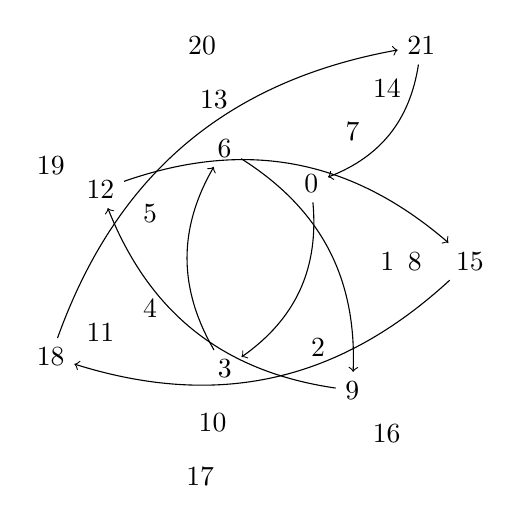
\begin{tikzpicture}[->,scale=.7]
   \node (a0) at (51.42:1.8cm)  {$0$};
   \node (a6) at (102.42:2.1cm) {$6$};
   \node (a5) at (154.26:2cm) {$5$};
   \node (a4) at (205.68:2cm)  {$4$};
   \node (a3) at (257.1:2cm) {$3$};
   \node (a2) at (308.52:2cm) {$2$};
   \node (a1) at (359.94:2.5cm)  {$1$};
   
   
   \node (a7) at (51.42:3cm)  {$7$};
   \node (a13) at (102.42:3cm) {$13$};
   \node (a12) at (154.26:3cm) {$12$};
   \node (a11) at (205.68:3cm)  {$11$};
   \node (a10) at (257.1:3cm) {$10$};
   \node (a9) at (308.52:3cm) {$9$};
   \node (a8) at (359.94:3cm)  {$8$};
   
   
   
   \node (a14) at (51.42:4cm)  {$14$};
   \node (a20) at (102.42:4cm) {$20$};
   \node (a19) at (154.26:4cm) {$19$};
   \node (a18) at (205.68:4cm)  {$18$};
   \node (17) at (257.1:4cm) {$17$};
   \node (a16) at (308.52:4cm) {$16$};
   \node (a15) at (359.94:4cm)  {$15$};
   \node (a21) at (51.42:5cm)  {$21$};

    \path (a0) edge[bend left] (a3);
   \path (a3) edge[bend left] (a6);
   \path (a6) edge[bend left] (a9);
   \path (a9) edge[bend left] (a12);
   \path (a12) edge[bend left] (a15);
   \path (a15) edge[bend left] (a18);
   \path (a18) edge[bend left] (a21);
   
   \path (a21) edge[bend left] (a0);

  
   \end{tikzpicture}\\\
\end{center}
$|3|$ = $\frac{l.c.m (3,7)}{3} ={\frac{21}{3}} = 7$\\\\
\begin{center}
    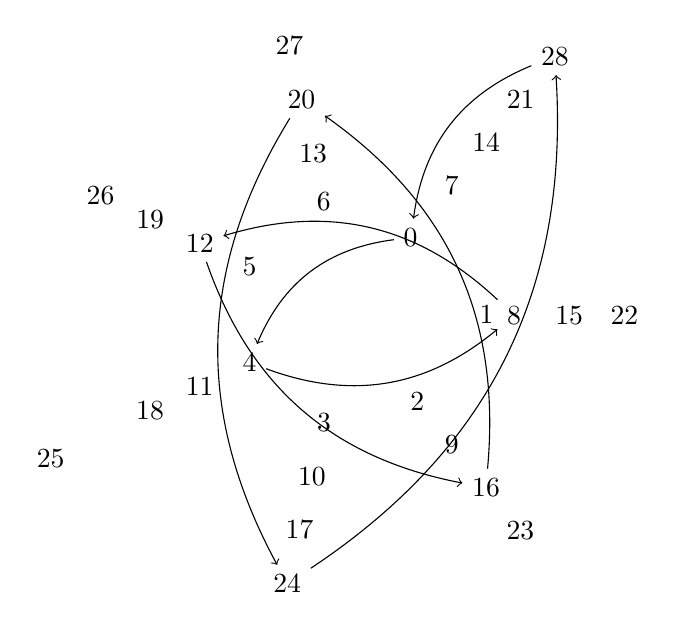
\begin{tikzpicture}[->,scale=.7]
   \node (a0) at (51.42:1.8cm)  {$0$};
   \node (a6) at (102.42:2.1cm) {$6$};
   \node (a5) at (154.26:2cm) {$5$};
   \node (a4) at (205.68:2cm)  {$4$};
   \node (a3) at (257.1:2cm) {$3$};
   \node (a2) at (308.52:2cm) {$2$};
   \node (a1) at (359.94:2.5cm)  {$1$};
   
   
   \node (a7) at (51.42:3cm)  {$7$};
   \node (a13) at (102.42:3cm) {$13$};
   \node (a12) at (154.26:3cm) {$12$};
   \node (a11) at (205.68:3cm)  {$11$};
   \node (a10) at (257.1:3cm) {$10$};
   \node (a9) at (308.52:3cm) {$9$};
   \node (a8) at (359.94:3cm)  {$8$};
   
   
   
   \node (a14) at (51.42:4cm)  {$14$};
   \node (a20) at (102.42:4cm) {$20$};
   \node (a19) at (154.26:4cm) {$19$};
   \node (a18) at (205.68:4cm)  {$18$};
   \node (17) at (257.1:4cm) {$17$};
   \node (a16) at (308.52:4cm) {$16$};
   \node (a15) at (359.94:4cm)  {$15$};
   \node (a21) at (51.42:5cm)  {$21$};

   \node (a27) at (102.42:5cm) {$27$};
   \node (a26) at (154.26:5cm) {$26$};
   \node (a25) at (205.68:6cm)  {$25$};
   \node (a24) at (257.1:5cm) {$24$};
   \node (a23) at (308.52:5cm) {$23$};
   \node (a22) at (359.94:5cm)  {$22$};
    \node (a28) at (51.42:6cm)  {$28$};


    \path (a0) edge[bend right] (a4);
   \path (a4) edge[bend right] (a8);
   \path (a8) edge[bend right] (a12);
   \path (a12) edge[bend right] (a16);
   \path (a16) edge[bend right] (a20);
   \path (a20) edge[bend right] (a24);
   \path (a24) edge[bend right] (a28);
   
   \path (a28) edge[bend right] (a0);

  
   \end{tikzpicture}\\\
\end{center}
$|4|$ = $\frac{l.c.m (4,7)}{4} ={\frac{28}{4}} = 7$\\\\
\begin{center}
    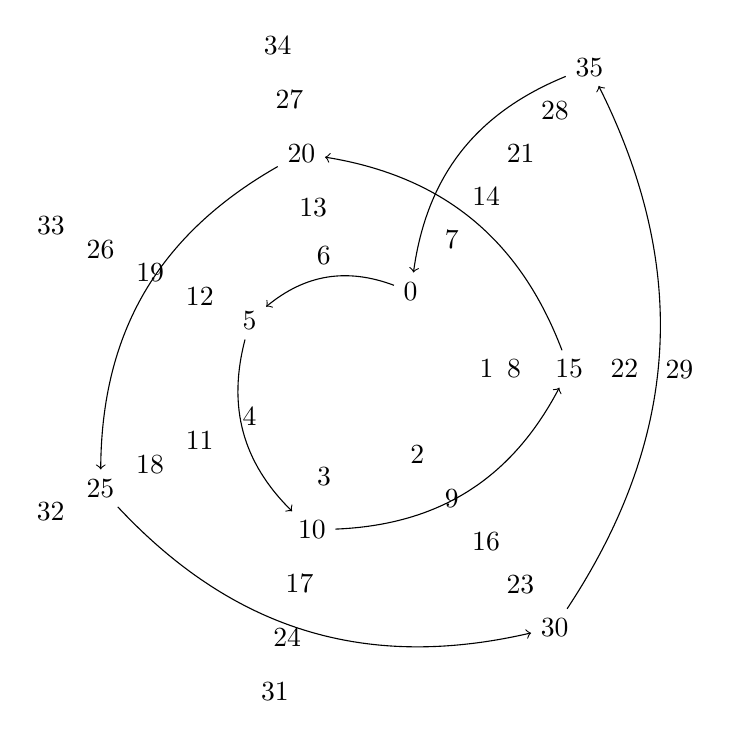
\begin{tikzpicture}[->,scale=.7]
   \node (a0) at (51.42:1.8cm)  {$0$};
   \node (a6) at (102.42:2.1cm) {$6$};
   \node (a5) at (154.26:2cm) {$5$};
   \node (a4) at (205.68:2cm)  {$4$};
   \node (a3) at (257.1:2cm) {$3$};
   \node (a2) at (308.52:2cm) {$2$};
   \node (a1) at (359.94:2.5cm)  {$1$};
   
   
   \node (a7) at (51.42:3cm)  {$7$};
   \node (a13) at (102.42:3cm) {$13$};
   \node (a12) at (154.26:3cm) {$12$};
   \node (a11) at (205.68:3cm)  {$11$};
   \node (a10) at (257.1:3cm) {$10$};
   \node (a9) at (308.52:3cm) {$9$};
   \node (a8) at (359.94:3cm)  {$8$};
   
   
   
   \node (a14) at (51.42:4cm)  {$14$};
   \node (a20) at (102.42:4cm) {$20$};
   \node (a19) at (154.26:4cm) {$19$};
   \node (a18) at (205.68:4cm)  {$18$};
   \node (17) at (257.1:4cm) {$17$};
   \node (a16) at (308.52:4cm) {$16$};
   \node (a15) at (359.94:4cm)  {$15$};
   \node (a21) at (51.42:5cm)  {$21$};

   \node (a27) at (102.42:5cm) {$27$};
   \node (a26) at (154.26:5cm) {$26$};
   \node (a25) at (205.68:5cm)  {$25$};
   \node (a24) at (257.1:5cm) {$24$};
   \node (a23) at (308.52:5cm) {$23$};
   \node (a22) at (359.94:5cm)  {$22$};
    \node (a28) at (51.42:6cm)  {$28$};


     
   
  \node (a29) at (359.94:6cm)  {$29$};
   \node (a30) at (308.52:6cm) {$30$};
   \node (a31) at (257.1:6cm) {$31$};
    \node (a32) at (205.68:6cm)  {$32$};
   \node (a33) at (154.26:6cm) {$33$};
   \node (a34) at (102.42:6cm) {$34$};
    \node (a35) at (51.42:7cm)  {$35$};


    \path (a0) edge[bend right] (a5);
   \path (a5) edge[bend right] (a10);
   \path (a10) edge[bend right] (a15);
   \path (a15) edge[bend right] (a20);
   \path (a20) edge[bend right] (a25);
   \path (a25) edge[bend right] (a30);
   \path (a30) edge[bend right] (a35);
   
   \path (a35) edge[bend right] (a0);

  
   \end{tikzpicture}\\\
\end{center}
$|5|$ = $\frac{l.c.m (5,7)}{5} ={\frac{35}{5}} = 7$\\\\
\begin{center}
    \begin{tikzpicture}[->,scale=.7]
   \node (a0) at (51.42:1.8cm)  {$0$};
   \node (a6) at (102.42:2.1cm) {$6$};
   \node (a5) at (154.26:2cm) {$5$};
   \node (a4) at (205.68:2cm)  {$4$};
   \node (a3) at (257.1:2cm) {$3$};
   \node (a2) at (308.52:2cm) {$2$};
   \node (a1) at (359.94:2.5cm)  {$1$};
   
   
   \node (a7) at (51.42:3cm)  {$7$};
   \node (a13) at (102.42:3cm) {$13$};
   \node (a12) at (154.26:3cm) {$12$};
   \node (a11) at (205.68:3cm)  {$11$};
   \node (a10) at (257.1:3cm) {$10$};
   \node (a9) at (308.52:3cm) {$9$};
   \node (a8) at (359.94:3cm)  {$8$};
   
   
   
   \node (a14) at (51.42:4cm)  {$14$};
   \node (a20) at (102.42:4cm) {$20$};
   \node (a19) at (154.26:4cm) {$19$};
   \node (a18) at (205.68:4cm)  {$18$};
   \node (17) at (257.1:4cm) {$17$};
   \node (a16) at (308.52:4cm) {$16$};
   \node (a15) at (359.94:4cm)  {$15$};
   \node (a21) at (51.42:5cm)  {$21$};

   \node (a27) at (102.42:5cm) {$27$};
   \node (a26) at (154.26:5cm) {$26$};
   \node (a25) at (205.68:5cm)  {$25$};
   \node (a24) at (257.1:5cm) {$24$};
   \node (a23) at (308.52:5cm) {$23$};
   \node (a22) at (359.94:5cm)  {$22$};
    \node (a28) at (51.42:6cm)  {$28$};


     
   
  \node (a29) at (359.94:6cm)  {$29$};
   \node (a30) at (308.52:6cm) {$30$};
   \node (a31) at (257.1:6cm) {$31$};
    \node (a32) at (205.68:6cm)  {$32$};
   \node (a33) at (154.26:6cm) {$33$};
   \node (a34) at (102.42:6cm) {$34$};
    \node (a35) at (51.42:7cm)  {$35$};


     \node (a36) at (359.94:7cm)  {$36$};
   \node (a37) at (308.52:7cm) {$37$};
   \node (a38) at (257.1:7cm) {$38$};
    \node (a39) at (205.68:7cm)  {$39$};
   \node (a40) at (154.26:7cm) {$40$};
   \node (a41) at (102.42:7cm) {$41$};
    \node (a42) at (51.42:8cm)  {$42$};


    \path (a0) edge[bend right] (a6);
   \path (a6) edge[bend right] (a12);
   \path (a12) edge[bend right] (a18);
   \path (a18) edge[bend right] (a24);
   \path (a24) edge[bend right] (a30);
   \path (a30) edge[bend right] (a36);
   \path (a36) edge[bend right] (a42);
   
   \path (a42) edge[bend right] (a0);

  
   \end{tikzpicture}\\\
\end{center}


$|6|$ = $\frac{l.c.m (6,7)}{6} ={\frac{42}{6}} = 7$\\\\

Here we can see if $Z_n$ if $n$ is a prime number the residue classes number or the elements are relatively prime to $n$ so the order number is always $n$.

Now lets take $Z_k$ So the elements are $Z_k$=$\{[0],[1],[2],[3],[4],[5],[6],.....,[(k-1)]$\} so the order of each element is \\\\
\begin{center}
    \begin{tikzpicture}[->,scale=1.2]
   \node (a) at (24:2cm)  {$2$};
   \node (b) at (48:2cm) {$1$};
   \node (c) at (72:2cm) {$0$};
   \node (d) at (96:2cm)  {$k-1$};
   \node (e) at (120:2cm) {$k-2$};
   \node (f) at (140:2cm) {$.$};
   \node (g) at (144:2cm)  {$.$};
   \node (q) at (148:2cm) {$.$};
   \node (r) at (152:2cm)  {$.$};
   \node (f) at (156:2cm) {$.$};
   \node (g) at (160:2cm)  {$.$};
   \node (q) at (164:2cm) {$.$};
   \node (r) at (168:2cm)  {$.$};
   \node (f) at (172:2cm) {$.$};
   \node (g) at (176:2cm)  {$.$};
   \node (q) at (180:2cm) {$.$};
   \node (r) at (184:2cm)  {$.$};
   \node (r) at (188:2cm)  {$.$};
   \node (h) at (192:2cm) {$10$};
   \node (i) at (216:2cm) {$9$};
   \node (j) at (240:2cm) {$8$};
   \node (k) at (264:2cm)  {$7$};
   \node (l) at (288:2cm) {$6$};
   \node (m) at (312:2cm) {$5$};
   \node (n) at (336:2cm)  {$4$};
   \node (o) at (360:2cm) {$3$};
   \node (p) at (72:2.5cm) {$k$};
   
   \end{tikzpicture}\\\
\end{center}

$|1|$ = $\frac{l.c.m (1,k)}{1}  $\\\\
$|2|$ = $\frac{l.c.m (2,k)}{2}  $\\\\
$|3|$ = $\frac{l.c.m (3,k)}{3}  $\\\\
$|4|$ = $\frac{l.c.m (4,k)}{4}  $\\\\
$|5|$ = $\frac{l.c.m (5,k)}{5}  $\\\\
$|6|$ = $\frac{l.c.m (6,k)}{6}  $\\\\
$|7|$ = $\frac{l.c.m (7,k)}{7}  $\\\\
$|8|$ = $\frac{l.c.m (8,k)}{8}  $\\\\
$|9|$ = $\frac{l.c.m (9,k)}{9}  $\\\\
.\\
.\\
.\\
.\\
.\\
.\\
$|k-2|$ = $\frac{l.c.m (k-2,k)}{k-2}   $\\\\
$|k-1|$ = $\frac{l.c.m (k-1,k)}{k} $\\\\
Here it is true for $Z_k$.We need to see now is it true for $Z_{k+1}$.\\\\
Let's take $Z_{K+1}$ so the residue classes are  $Z_{k+1}$=$\{[0],[1],[2],[3],[4],[5],[6],.....,[((k+1)-2)],[((k+1)-1)]$\}\\\\
$Z_{k+1}$=$\{[0],[1],[2],[3],[4],[5],[6],.....,[((k-1)],[((k)]$\}\\\\\
\begin{center}
    \begin{tikzpicture}[->,scale=1.2]
   \node (a) at (24:2cm)  {$2$};
   \node (b) at (48:2cm) {$1$};
   \node (c) at (72:2cm) {$0$};
   \node (d) at (96:2cm)  {$k$};
   \node (e) at (120:2cm) {$k-1$};
   \node (f) at (140:2cm) {$.$};
   \node (g) at (144:2cm)  {$.$};
   \node (q) at (148:2cm) {$.$};
   \node (r) at (152:2cm)  {$.$};
   \node (f) at (156:2cm) {$.$};
   \node (g) at (160:2cm)  {$.$};
   \node (q) at (164:2cm) {$.$};
   \node (r) at (168:2cm)  {$.$};
   \node (f) at (172:2cm) {$.$};
   \node (g) at (176:2cm)  {$.$};
   \node (q) at (180:2cm) {$.$};
   \node (r) at (184:2cm)  {$.$};
   \node (r) at (188:2cm)  {$.$};
   \node (h) at (192:2cm) {$10$};
   \node (i) at (216:2cm) {$9$};
   \node (j) at (240:2cm) {$8$};
   \node (k) at (264:2cm)  {$7$};
   \node (l) at (288:2cm) {$6$};
   \node (m) at (312:2cm) {$5$};
   \node (n) at (336:2cm)  {$4$};
   \node (o) at (360:2cm) {$3$};
   \node (p) at (72:2.5cm) {$k+1$};
   
   \end{tikzpicture}\\\
\end{center}

$|1|$ = $\frac{l.c.m (1,k+1)}{1}  $\\\\
$|2|$ = $\frac{l.c.m (2,k+1)}{2}  $\\\\
$|3|$ = $\frac{l.c.m (3,k+1)}{3}  $\\\\
$|4|$ = $\frac{l.c.m (4,k+1)}{4}  $\\\\
$|5|$ = $\frac{l.c.m (5,k+1)}{5}  $\\\\
$|6|$ = $\frac{l.c.m (6,k+1)}{6}  $\\\\
$|7|$ = $\frac{l.c.m (7,k+1)}{7}  $\\\\
$|8|$ = $\frac{l.c.m (8,k+1)}{8}  $\\\\
$|9|$ = $\frac{l.c.m (9,k+1)}{9}  $\\\\
.\\
.\\
.\\
.\\
.\\
.\\
$|k-1|$ = $\frac{l.c.m (k-1,k+1)}{k-1}   $\\\\
$|k|$        = $\frac{l.c.m (k,k+1)}{k} $\\\\
The order of $|0|$ is always $1$\\\
Here,We can clearly see the $k$ and $(k+1)$ are two consecutive numbers so they are co-primes,so $k^{th}$ order is always $(k+1)$.Hence this is true for any numbers.\\\
The order of element $a$ in $Z_n$ is  ${\frac{l.c.m(a,n)}{a}}$ where $0<a\le n-1$.
\subsubsection{Corollary}
We can clearly see that the order of $|0|$ is always $1$ in this situation.\\
and when the element number $a$ and the number addition modulo $Z_n$ is relative prime then the order is $n$.and Any two consecutive integers or numbers will always be Co-Prime numbers since the successive numbers’ GCD will be always $1$. Example: $\{1,2\}, \{2,3\}, \{3,4\}, \{4,5\}, \{5,6\}$ and so on.So it is true for $Z_k$.
\section{The Code}
\subsection{The process}
We use Visual Studio Code as a compiler and for coding environment we choose python 3.14 version to produce the code.here we attach a picture of it and its true for any number in addition modulo of $Z_n$.This is for local computer version here the output will save into the local folder.We can see the output in a text file.\\\\
\includegraphics[width=.8\linewidth]{abcd.png}\\\
If the order of the elements are repeating we can conclude that the $Z_n$ where n is any prime number.\\\
\subsection{Source Code :}
\begin{lstlisting}[language=Python, caption=Python example]
def lcm(x, y):

   if x > y:
       maximum_num = x
   else:
       maximum_num = y

   while(True):
       if((maximum_num % x == 0) and (maximum_num % y == 0)):
           lcm = maximum_num
           break
       maximum_num += 1

   return lcm
n=int(input("Enter the Addition Modulo nummber n: "))

#with open('Additionmodulo.txt',"wt") as ft:
print("The vule of n  is ",n)#,file=ft)
print("The order of  0  is  =  1.0 ")
print("so the order of the elements are 1 to", n-1)#,file=ft)
#The order of 0 is going to be always 1

for i in range(1,n):

    order= lcm(i,n)/i 
        #Here order is the formula to find the order of an element 
        #in a group under addition modulo.
    
    print("The order of ",i," is  = ",order)#,file=ft)
    


    
\end{lstlisting}
\subsection{The Output}
When this program is executed, the results are:
\begin{lstlisting}[language=Python, caption=Python output]
Enter the Addition Modulo nummber n:
100
The value of n  is  100
The order of  0  is  =  1.0 
so the order of the elements are 1 to 99
The order of  1  is  =  100.0
The order of  2  is  =  50.0
The order of  3  is  =  100.0
The order of  4  is  =  25.0
The order of  5  is  =  20.0
The order of  6  is  =  50.0
The order of  7  is  =  100.0
The order of  8  is  =  25.0
The order of  9  is  =  100.0
The order of  10  is  =  10.0
The order of  11  is  =  100.0
The order of  12  is  =  25.0
The order of  13  is  =  100.0
The order of  14  is  =  50.0
The order of  15  is  =  20.0
The order of  16  is  =  25.0
The order of  17  is  =  100.0
The order of  18  is  =  50.0
The order of  19  is  =  100.0
The order of  20  is  =  5.0
The order of  21  is  =  100.0
The order of  22  is  =  50.0
The order of  23  is  =  100.0
The order of  24  is  =  25.0
The order of  25  is  =  4.0
The order of  26  is  =  50.0
The order of  27  is  =  100.0
The order of  28  is  =  25.0
The order of  29  is  =  100.0
The order of  30  is  =  10.0
The order of  31  is  =  100.0
The order of  32  is  =  25.0
The order of  33  is  =  100.0
The order of  34  is  =  50.0
The order of  35  is  =  20.0
The order of  36  is  =  25.0
The order of  37  is  =  100.0
The order of  38  is  =  50.0
The order of  39  is  =  100.0
The order of  40  is  =  5.0
The order of  41  is  =  100.0
The order of  42  is  =  50.0
The order of  43  is  =  100.0
The order of  44  is  =  25.0
The order of  45  is  =  20.0
The order of  46  is  =  50.0
The order of  47  is  =  100.0
The order of  48  is  =  25.0
The order of  49  is  =  100.0
The order of  50  is  =  2.0
The order of  51  is  =  100.0
The order of  52  is  =  25.0
The order of  53  is  =  100.0
The order of  54  is  =  50.0
The order of  55  is  =  20.0
The order of  56  is  =  25.0
The order of  57  is  =  100.0
The order of  58  is  =  50.0
The order of  59  is  =  100.0
The order of  60  is  =  5.0
The order of  61  is  =  100.0
The order of  62  is  =  50.0
The order of  63  is  =  100.0
The order of  64  is  =  25.0
The order of  65  is  =  20.0
The order of  66  is  =  50.0
The order of  67  is  =  100.0
The order of  68  is  =  25.0
The order of  69  is  =  100.0
The order of  70  is  =  10.0
The order of  71  is  =  100.0
The order of  72  is  =  25.0
The order of  73  is  =  100.0
The order of  74  is  =  50.0
The order of  75  is  =  4.0
The order of  76  is  =  25.0
The order of  77  is  =  100.0
The order of  78  is  =  50.0
The order of  79  is  =  100.0
The order of  80  is  =  5.0
The order of  81  is  =  100.0
The order of  82  is  =  50.0
The order of  83  is  =  100.0
The order of  84  is  =  25.0
The order of  85  is  =  20.0
The order of  86  is  =  50.0
The order of  87  is  =  100.0
The order of  88  is  =  25.0
The order of  89  is  =  100.0
The order of  90  is  =  10.0
The order of  91  is  =  100.0
The order of  92  is  =  25.0
The order of  93  is  =  100.0
The order of  94  is  =  50.0
The order of  95  is  =  20.0
The order of  96  is  =  25.0
The order of  97  is  =  100.0
The order of  98  is  =  50.0
The order of  99  is  =  100.0



\end{lstlisting}
Its written for Online Python-3 Compiler (Interpreter).We can check for any value and it is true\\
This code is for any $k_{th}$ element's order where $k\geq1$.


\section{Conclusion}
We use multiple number theory concepts to solve the order of an element in a group under addition modulo, and this gives us another way to determine whether a number is prime or not.To observe modular arithmetic, we use a wheel setup..This is The Generalization form of order of an
element in a group under addition
modulo.


% \section*{Acknowledgement}
% I'd like to thank my Professor \textbf{Dr Chandrani Nag} for advising me and guiding me in the right direction. This would have been impossible without her.\\\
% Contacts : \textbf{Dr Chandrani Nag, Professor}\\\
% Department of Mathematics, Shahjalal University of Science and Technology, Sylhet, Bangladesh.\\\
% Email: nagbd@yahoo.com

















\bibliographystyle{plain}
\bibliography{references.bib}



\end{document}
